\chapter{In-depth component description}

\section{Communicating with Channels}

\texttt{Channel} is an interface for performing I/O operations. It represents the principal abstraction used by the middleware to communicate with hardware devices and external software services.

\lstset{language=Java}
\begin{lstlisting}[float,caption=The Channel interface,label={lst:channel}]
public interface Channel {

	public String getId();
	
	public IOTask submit(IORequest request, IOHandler handler)
			throws ChannelException;
	
	public void setAsyncIOHandler(IOHandler handler)
			throws IllegalStateException;
			
	public boolean isClosed();
	
	public void close();
			
}
\end{lstlisting}

The \texttt{Channel} interface is not tied to any specific technology or communication stack; as a result of this design choice, a wide variety of data management tasks, including but not limited to, networking, file handling, and automatic data generation can be implemented as \texttt{Channel}s.

The current middleware architecture encourages the creation of several highly specialized \texttt{Channel}s, which are usually developed around third-party communication libraries. \texttt{HTTPChannel}, a \texttt{Channel} providing support for HTTP communications, is an excellent example of the advantages of this design strategy. Implemented as a simple wrapper around Apache's HTTP Components toolkit, its development only required a basic understanding of the HTTP protocol; yet \texttt{HTTPChannel} is a fully compliant HTTP/1.1 client (see section~\ref{sec:channel.implementations} for additional details).

Upon instantiation, \texttt{Channel}s are open and ready to be used. They may be optionally closed to relinquish unused resources by invoking the \texttt{close()} method. Once closed, a \texttt{Channel} cannot be re-opened, and every subsequent attempt to perform an I/O operation will fail causing a \texttt{ChannelException} to be thrown. The current state of a \texttt{Channel} can be probed through its \texttt{isClosed()} method.

Bytes sent or received with a \texttt{Channel} are encapsulated within a \texttt{Payload}, an object whose interface (listing~\ref{lst:payload}) allows \texttt{Channel}s and other data manipulation components to handle different data types regardless of the particular data representation chosen by the Middleware. \texttt{Payload}s will be the subject of further discussion in section~\ref{sec:components.mapper}

\lstset{language=Java}
\begin{lstlisting}[float,caption=The Payload interface,label={lst:payload}]
public interface Payload {

	public Charset getCharset();

	public InputStream asInputStream();

	public ByteBuffer asByteBuffer();

	public String asString();

}
\end{lstlisting}

All user-initiated I/O operations begin with an invocation of the \texttt{Channel.submit()} method. As can be seen in listing~\ref{lst:channel}, \texttt{submit()} is a direct implementation of the asynchronous interaction paradigm introduced in section~\ref{sec:newmiddleware.async}.

The emphasis on asynchronous execution is underscored by the absence of blocking operations in the \texttt{Channel} interface. This aspect is of paramount importance for the entire Middleware design, as implementing a truly asynchronous system would prove impossible if such feature were not provided by its core data access layer.


\section{Instantiating Channels}

Creation of new \texttt{Channel}s is performed by means of the  \texttt{ChannelFactory} interface, a reification of the Factory design pattern that allows polymorphic instantiation of object classes.

By using the Factory instantiation model, the choice of a particular \texttt{Channel} implementation can be postponed from compile time to run time. This technique allows the Middleware to dynamically adapt in response to environment changes, and to support extension through the addition of new user-defined \texttt{Channel}s. For further information regarding the Factory pattern and its uses inside the PerLa Middleware, refer to section~\ref{sec:newmiddleware.factory}.

All data required to create a new \texttt{Channel} must be stored inside a \texttt{ChannelDescriptor}. As shown in listing~\ref{lst:channelFactory}, this configuration object is the only parameter required to correctly invoke the \texttt{createChannel()} method.

\lstset{language=Java}
\begin{lstlisting}[float,caption=The ChannelFactory interface,label={lst:channelFactory}]
public interface ChannelFactory {

	public Class<? extends ChannelDescriptor>
			acceptedChannelDescriptorClass();

	public Channel createChannel(ChannelDescriptor descriptor)
			throws InvalidDeviceDescriptorException;

}
\end{lstlisting}

\begin{figure}[h!]
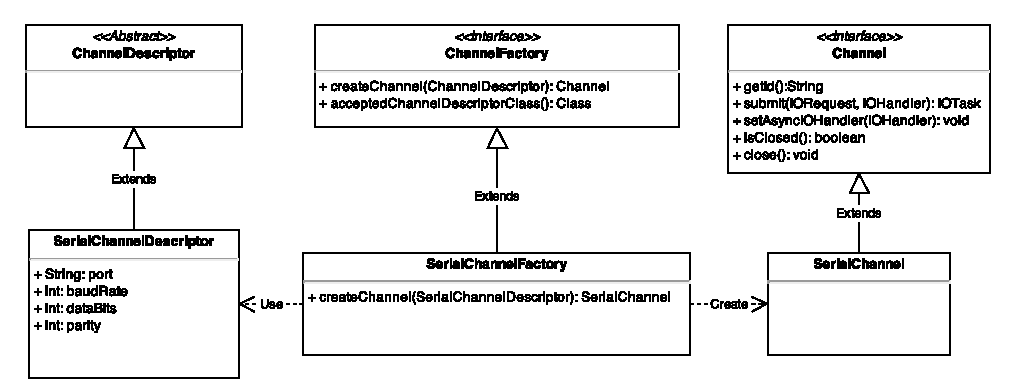
\includegraphics[width=\textwidth]{imgs/channel_factory.pdf}
\caption{Class diagram of the Channel layer}
\end{figure}

Each \texttt{ChannelFactory} is tied to a specific communication technology; therefore, it can only accept a single class of \texttt{ChannelDescriptor} objects. For example, the \texttt{HTTPChannelFactory} parses \texttt{HTTPChannelDescriptor}s and creates \texttt{HTTPChannel}s, whereas the hypothetical \texttt{SerialChannelFactory} would consume \texttt{SerialChannelDescriptor}s to create \texttt{SerialChannel}s. Failure to provide a suitable \texttt{ChannelDescriptor} object will cause the \texttt{createChannel()} method to throw an \texttt{InvalidDeviceDescriptorException}.

The \texttt{acceptedChannelDescriptorClass()} method can be used to dynamically discover which \texttt{ChannelDescriptor} type is supported by a specific \texttt{ChannelFactory}. This method is the fulcrum of the \texttt{Channel} Plugin System, as it allows the Middleware to invoke the most appropriate \texttt{ChannelFactory} using only information available at runtime.

\begin{figure}[!hbt]
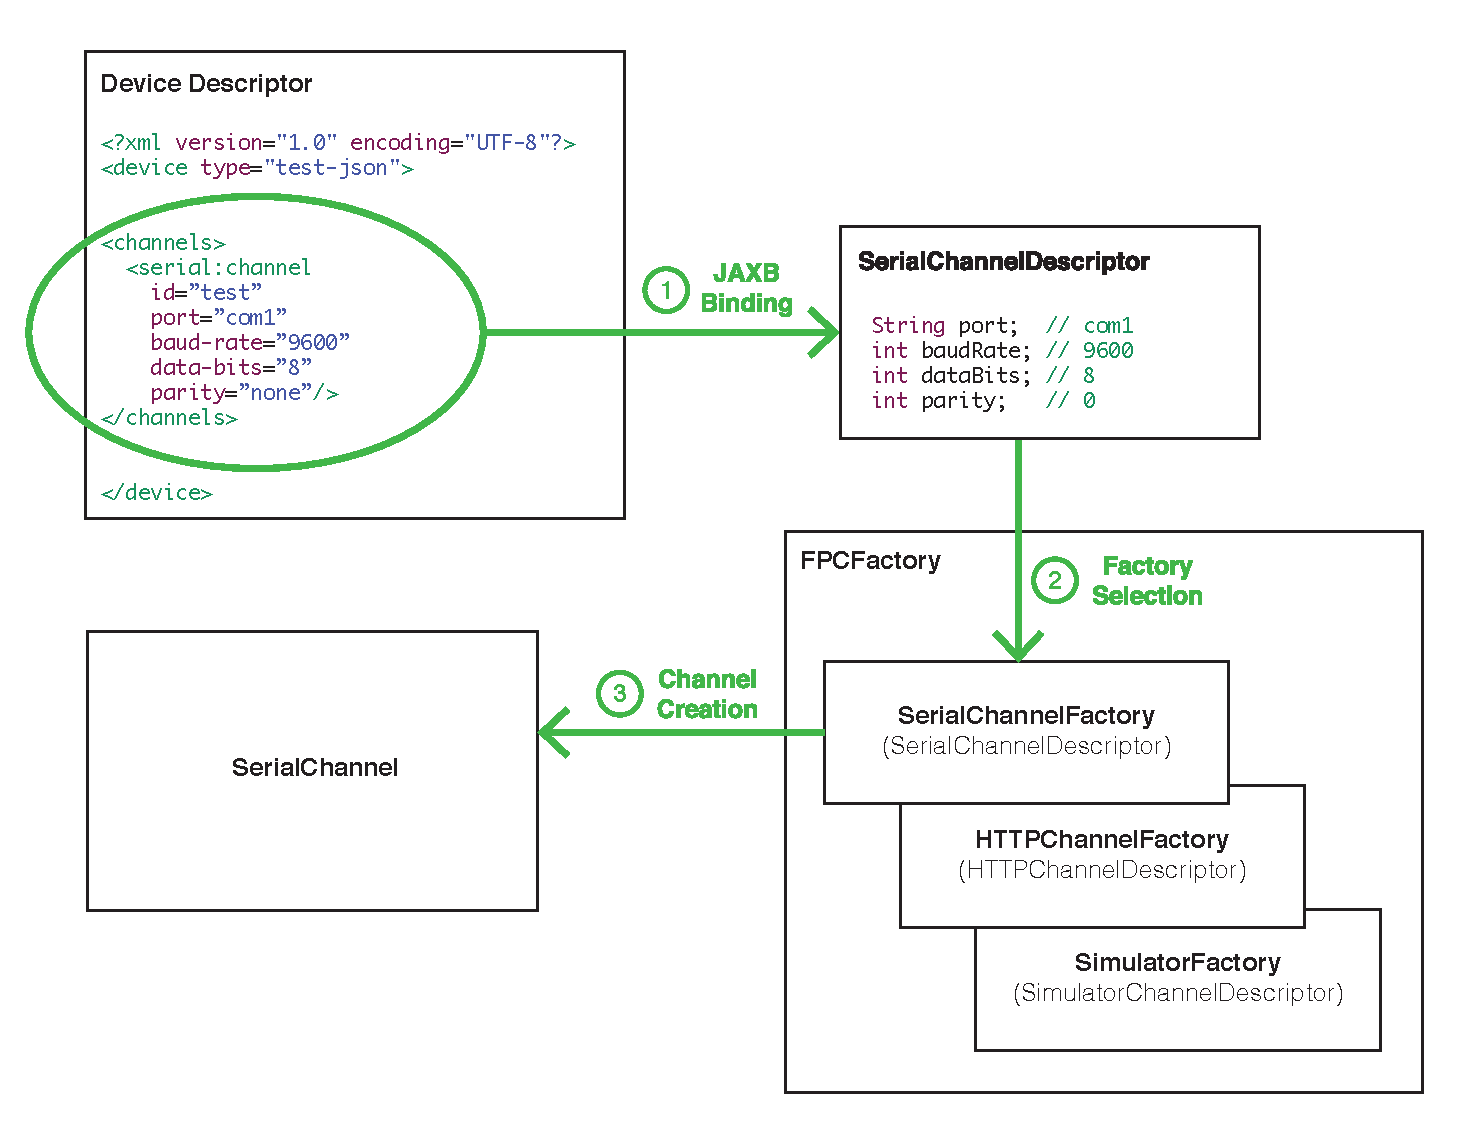
\includegraphics[width=\textwidth]{imgs/channel_creation_process.pdf}
\caption{The Channel creation process}
\label{fig:channel.creation}
{
\begin{figurenote}
This figure illustrates the \texttt{Channel} creation process executed by the Middleware upon reception of a new Device Descriptor.
\begin{enumerate}
  \itemsep0em
  \item JAXB binds the XML Device Descriptor to an apropriate \texttt{ChannelDescriptor} object using namespace information
  \item A suitable \texttt{ChannelFactory} is selected at runtime using the \texttt{acceptedChannelDescriptorClass()} method
  \item The information contained in the \texttt{SerialChannelDescriptor} is used to create a new \texttt{SerialChannel}
\end{enumerate}
\vspace{-1em}
\end{figurenote}
}
\end{figure}

\texttt{ChannelDescriptor} objects are automatically instantiated by the Middleware using the information contained in the Device Descriptor XML files. This binding process is automatically performed by the JAXB library, which is also responsible for instantiating the correct \texttt{ChannelDescriptor} class using XML Namespace information. Figure~\ref{fig:channel.creation} provides a visual example of this technique, and ties it together with the other operations described in this section.

It is important to note that a single JVM instance running the PerLa Middleware may host several \texttt{Channel} objects of the same type, at the same time. Several devices can use the same communication technology, and the \texttt{ChannelFactory} may determine that it's best to create an individual \texttt{Channel} for each one of them. This behaviour is fostered by the new \texttt{ChannelFactory} architecture, and is considered idiomatic design; hence, it would not be uncommon to implement the hypothetical \texttt{SerialChannelFactory} introduced in the previous paragraphs so that every serial port is handled by a different \texttt{SerialChannel} instance.


\subsection{IORequest management}

\texttt{IORequest} is the base object interface employed to interact with a device connected to the Middleware. It contains two types of information: the payload to be transferred, and \texttt{Channel}-dependent data needed for a correct communication with the endpoint device.

\lstset{language=Java}
\begin{lstlisting}[float,floatplacement=!hbt,caption=The IORequest interface,label={lst:iorequest}]
public interface IORequest {

	public String getId();

	public void setParameter(String name, Payload payload);
	
}
\end{lstlisting}

Since different communication technologies require different configuration settings to establish end-to-end connectivity, every \texttt{Channel} is bundled with one or more custom \texttt{IORequest} classes. Following up on previous examples, the \texttt{HTTPChannel} package contains a \texttt{HTTPIORequest} object, whereas the fictitious \texttt{SerialChannel} would be supplied with a \texttt{SerialIORequest} class of request objects.

As shown in listing~\ref{lst:iorequest}, payload data can be set in an \texttt{IORequest} by means of the \texttt{setParameter()} method. \texttt{Payload}s are addressed by name, and a single \texttt{IORequest} implementation may support several at once. The exact set of \texttt{Payload} parameters accepted by an \texttt{IORequest} class depends on the design of the associated \texttt{Channel}; for example, the \texttt{HTTPChannel} implementation provided with the Middleware supports three: an `entity' payload (request body), a `query' payload (an URL-encoded string), and a `path' payload (a path component used to identify a single resource accessible from the base URL).

\texttt{IORequest}s are disposable objects; they are created, submitted to a \texttt{Channel}, and garbage collected once the communication is over. Creation is performed by means of a factory interface dubbed \texttt{IORequestBuilder}, which allows the Middleware to build new copies of an \texttt{IORequest} from a fixed template. It is important to note that request objects built using this technique do not contain any \texttt{Payload} parameter; these are to be added manually before subbmitting the \texttt{IORequest} to a \texttt{Channel}.

A single device connected to the PerLa Middleware is generally managed using several \texttt{IORequestBuilder}s, any one of which is responsible for creating requests that control a single aspect of the interaction with the endpoint. The main advantage brought by this templating mechanism is that \texttt{Channel}-related configuration settings are only specified once, hence the same \texttt{IORequest} structure can be reused multiple times to transport different payload information.

REST APIs are an excellent use case to demonstrate the aforementioned concept, as every operation on a RESTful resource can be easily abstracted using an appropriately configured request builder. By using \texttt{HTTPIORequestBuilder} objects, HTTP protocol information (base URL, method, header information, \ldots) are specified one single time only for every REST endpoint. Once this step is done, the API can be invoked just by building new \texttt{IORequest}s and submitting them to a \texttt{HTTPChannel}.

Besides \texttt{IORequest} creation, the \texttt{IORequestBuilder} interface can be used to dynamically discover all \texttt{Payload} parameters supported by an \texttt{IORequest}. This functionality, exposed through the \texttt{getParameterList()} method, is a crucial component of the Middleware Plugin System, as it allows \texttt{Script} instructions to determine whether an \texttt{IORequest} was correctly populated with all the necessary \texttt{Payload} parameters or not. This concept will be the subject of further analysis in section~\ref{sec:components.script}.

\begin{figure}[!hbt]
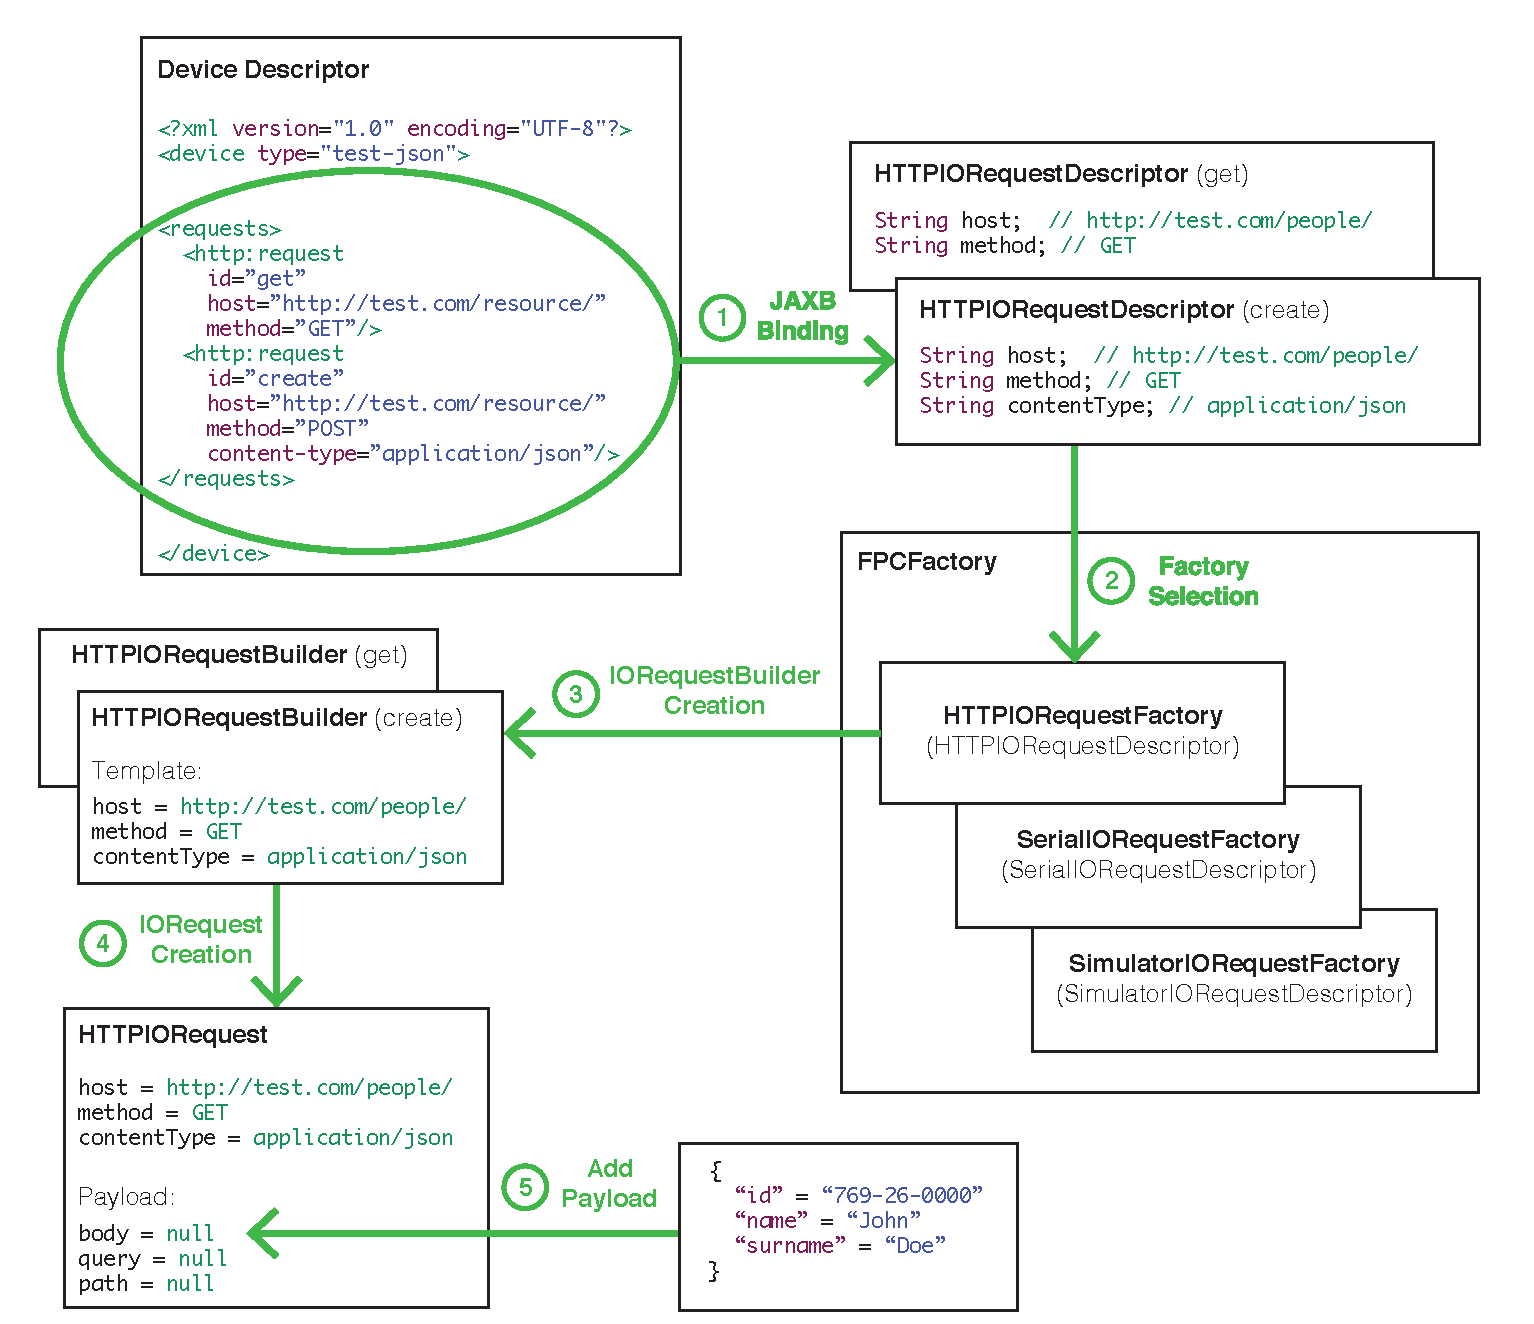
\includegraphics[width=\textwidth]{imgs/iorequest_creation_process.pdf}
\caption{The IORequest creation process}
\label{fig:iorequest.creation}
{
\begin{figurenote}
This figure illustrates the autonomous creation of \texttt{IORequest} objects. Steps 1 to 3 are performed only once after receiving the Device Descriptor, whereas steps 4 and 5 are repeated every time the REST API is to be invoked.
\begin{enumerate}
  \itemsep0em
  \item JAXB binds the XML Device Descriptor to an apropriate \texttt{IORequestDescriptor} object using namespace information
  \item A suitable \texttt{IORequestBuilderFactory} is selected at runtime using the \texttt{acceptedIORequestDescriptorClass()} method
  \item The information contained in the \texttt{IORequestDescriptor} is used to create a new \texttt{IORequestBuilder}
  \item The \texttt{IORequestBuilder} is used to create new \texttt{IORequest} copies using the internal template
  \item The newly created \texttt{IORequest} objects can be populated with \texttt{Payload} parameters as needed
\end{enumerate}
\vspace{-1em}
\end{figurenote}
}
\end{figure}

\texttt{IORequestBuilder}s are created by means of an \texttt{IORequestBuilderFactory}, an object that implements the now familiar Factory design pattern. Similarly to what already seen in the previous section, every \texttt{IORequestBuilderFactory} implements an \texttt{acceptedIORequestDescriptorClass()} method, which can be used to dynamically determine if a factory object can parse a specific type of \texttt{IORequestDescriptor}.   It should come as no surprise that every \texttt{IORequestBuilder} class should be provided with complementary \texttt{IORequestBuilderFactory} and \texttt{IORequestDescriptor} implementations.

Creation of a new \texttt{IORequestBuilder} object proceeds as follows: The template for creating new \texttt{IORequest} objects is loaded from an XML Device Descriptor, bound to an appropriate \texttt{IORequestDescriptor}, and processed by the \texttt{IORequestBuilderFactory} to create the corresponding \texttt{IORequestBuilder}. Figure~\ref{fig:iorequest.creation} provides a comprehensive overview on this process and on the management of \texttt{IORequest} objects.


\subsection{Handling asynchronous I/O operations}

The outcome of an I/O operation are collected through the \texttt{IOHandler} passed as parameter to the \texttt{submit()} method. 

\texttt{submit()} requires the caller to specify an \texttt{IOHandler} callback object, through which data and errors will be notified once the requested operation is complete.

The execution of an ongoing I/O operations can be monitored and altered using the \texttt{IOTask} object returned 






Every user-initiated interaction with a \texttt{Channel} begins with the creation of an appropriate \texttt{IORequest}, an object that contains all parameters required to characterize the I/O operation being started. Different \texttt{Channel}s require different \texttt{IORequest}s, since the parameters needed for starting an I/O operation depend upon the technical characteristics of the I/O operation itself.

Since the specific contents of an \texttt{IORequest} object vary with the type of , the middleware does not provide a universal implementation for the \texttt{IORequest} object, 


A class of \texttt{IORequest} objects is tipically designed to be used with a specific \texttt{Channel} implementation, as its contents strictly depend on the gamut of operations supported by the \texttt{Channel} by which it is supposed to be executed 

The specific contents of an this object depend on the type of operations supported by the \texttt{Channel} that will perform

Different communication tasks require different parameters to be performed successfully: an appropriate URL is needed 

It is clear, even from this short lists of examples, that different IORequest objects

As such, a class of \texttt{IORequest} objects is typically...

 A class of \texttt{IORequest} objects is tipically designed to be used with a specific \texttt{Channel} implementation, as its contents strictly depend on the gamut of operations supported by the \texttt{Channel} by which it is supposed to be executed (e.g., \texttt{HTTPIORequests} can only be processed by an \texttt{HTTPChannel}). For this reason, the middleware does not provide a default implementation is provided for the \texttt{IORequest} interface. A set of guidelines for the implementation and management of \texttt{IORequest} objects will follow in the next sections of this chapter.

\texttt{IORequest} objects can be submitted to a \texttt{Channel} by means of the \texttt{submit()} method. As can be seen in listing~\ref{lst:channel}, this method is a direct implementation of the asynchronous invocation paradigm introduced in section~\ref{sec:newmiddleware.async}. Calls to \texttt{submit()} are non-blocking and require the caller to specify an \texttt{IOHandler} callback object, through which data and errors will be notified once the requested operation is complete.

The status of an ongoing operation can be queried and modified with the \texttt{IOTask} object, which is returned upon submitting a new request.


\lstset{language=Java}
\begin{lstlisting}[float,floatplacement=H,caption=The IOHandler interface,label={lst:iohandler}]
public interface IOHandler {
	public void complete(IORequest request, Optional<Payload> result);
	
	public void error(IORequest request, Throwable cause);
}
\end{lstlisting}

\lstset{language=Java}
\begin{lstlisting}[float,floatplacement=H,caption=The IOTask interface,label={lst:iotask}]
public interface IOTask {
	public void cancel();
	
	public IORequest getRequest();
	
	public boolean isCancelled();
	
	public boolean isDone();
}
\end{lstlisting}







There is no limit on the number of channels used by an FPC. Complex behaviours can be implemented using different channels

Interface description: methods, IORequest, IOHandler IOTask and Payload.
ByteArrayPayload description

The new Channel structure is monolithic, in that it contains all network layers required for the communication. This is in contrast with the previous middleware architecture, where communication layers where diveded between the legacy Channel implementation and the FPC. This new structure allows better reuse of off-the-shelf libraries.

ChannelFactory interface, methods and generic ChannelDescriptor structure

Basic XML 

IORequestBuilder and IORequestBuilderFactory

setAsyncIOHandler, how does it work and why do we need it

\subsection{Implementations: HTTPChannel and SimulatorChannel}
\label{sec:channel.implementations}

Full examples of actual implementations, complete with XML descriptor snippets


\section{Encoding and decoding information}
\label{sec:components.mapper}

\subsection{The Message and Mapper interfaces}

\subsection{Handling composite data structures}

\subsection{Managing multiple message types}

\subsection{Implementations: JSONMapper and URLEncodedMapper}


\section{Data management: Scripts}
\label{sec:components.script}

\subsection{From Messages to Records}

\subsection{Available instructions}

\subsection{Engine architecture and execution model}

\subsection{Script examples}


\section{Putting it all together: the FPC}

\subsection{Data access interface}

\subsection{Controlling the remote device}

\subsection{Scheduling mechanism}


\section{Device Descriptor and FPC Factory}

\subsection{The XML Device Descriptor}

\subsection{FPC Factory}

\subsection{Registry}

\subsection{Complete XML Device Descriptor examples}